\section*{Introducción al fenómeno}

\textcolor{edit30sept}{Mi aproximación al Hospital San Juan de Dios no surge de una distancia académica convencional, sino de una intimidad familiar que inicialmente me mantuvo en una posición de “observador silente”. Esta condición particular, lejos de constituir una limitación metodológica, se revela como una perspectiva necesaria para comprender las complejidades visuales y emocionales del caso. Como señala Etienne Samain en su reflexión sobre el trabajo con archivos fotográficos, “acepta el desafío de efectivamente crear mecanismos originales de trabajo con las imágenes en la dirección de una anamnesis de su propia experiencia visual” (Samain, 2016, p. 116). En mi caso, esta anamnesis personal se convierte en herramienta epistemológica fundamental.}

\textcolor{edit30sept}{El vínculo directo con el San Juan —mi madre fue trabajadora del hospital— me posicionó inicialmente en lo que denomino un “pudor investigativo”: una resistencia ética a “meter la mano” en un conflicto que transformaba radicalmente la vida de las personas más cercanas. Este pudor, que posteriormente comprendí como una forma de respeto hacia la complejidad del fenómeno, se transformó gradualmente en curiosidad metodológica. La observación del cambio profundo en el estilo de vida de mi madre, su decisión moral y ética de formar parte del proceso de resistencia, me reveló que en el San Juan ocurrían eventos que demandaban “una mirada crítica” más allá de lo meramente político o laboral.}

\textcolor{edit30sept}{La investigación tomó un giro definitivo cuando Margarita Castro me ofreció acceso a su archivo personal —“sus discos, sus imágenes, sus fotografías”— en un gesto que Samain describe perfectamente: “ella no lo llama archivo, sino me comparte”. Este momento marca lo que podríamos denominar un “encuentro con la imagen del San Juan”: la búsqueda de respuestas en el “adentro” del hospital se resolvió en “otro momento, en otro espacio, en otro lugar, en otra materialidad que es en los archivos digitales y en los archivos físicos de Margarita”.}

\textcolor{edit30sept}{Como establece Samain en su metodología de trabajo con archivos visuales, el investigador debe preguntarse: “¿qué se pretende hacer de un archivo, cuáles serán sus destinos? ¿Para quién, como y por qué?” (Samain, 2016, p. 116). En el caso del archivo de Margarita, me encontré ante “una colección sin colección, un archivo sin archivo”: una mezcla de miradas que incluía tanto “la mirada de quien registra su propia historia” como “la mirada de quien indaga”. Esta multiplicidad de perspectivas contenidas en un mismo corpus visual evidencia lo que Samain denomina la “potencia” de las imágenes para hacer emerger significados que trascienden la intencionalidad original del registro.}

\textcolor{edit30sept}{El descubrimiento crucial fue comprender que “la imagen emerge no por capricho, sino porque la imagen está ahí latente, la imagen finalmente emerge ante el atractor de la mirada”. En el trabajo de artistas como David Lozano en su obra Hortúa Inhospitalaria (véase Figura~\ref{fig:david_lozano_hortua}), pude observar cómo confluían múltiples dimensiones: “el drama social, el drama laboral, también como la profundidad digamos del abandono arquitectónico, patrimonial, el tema del cuidado humano, el tema del cuerpo”. Esta confluencia reveló que las manifestaciones visuales y estéticas no eran superficiales, sino que operaban como condensadores de complejidades sociales más profundas.}

\begin{figure}[p]
    \thispagestyle{empty}
    \captionsetup{labelformat=empty,textformat=empty}
    \begin{tikzpicture}[remember picture,overlay]
        \node[inner sep=0pt] at (current page.center) {
            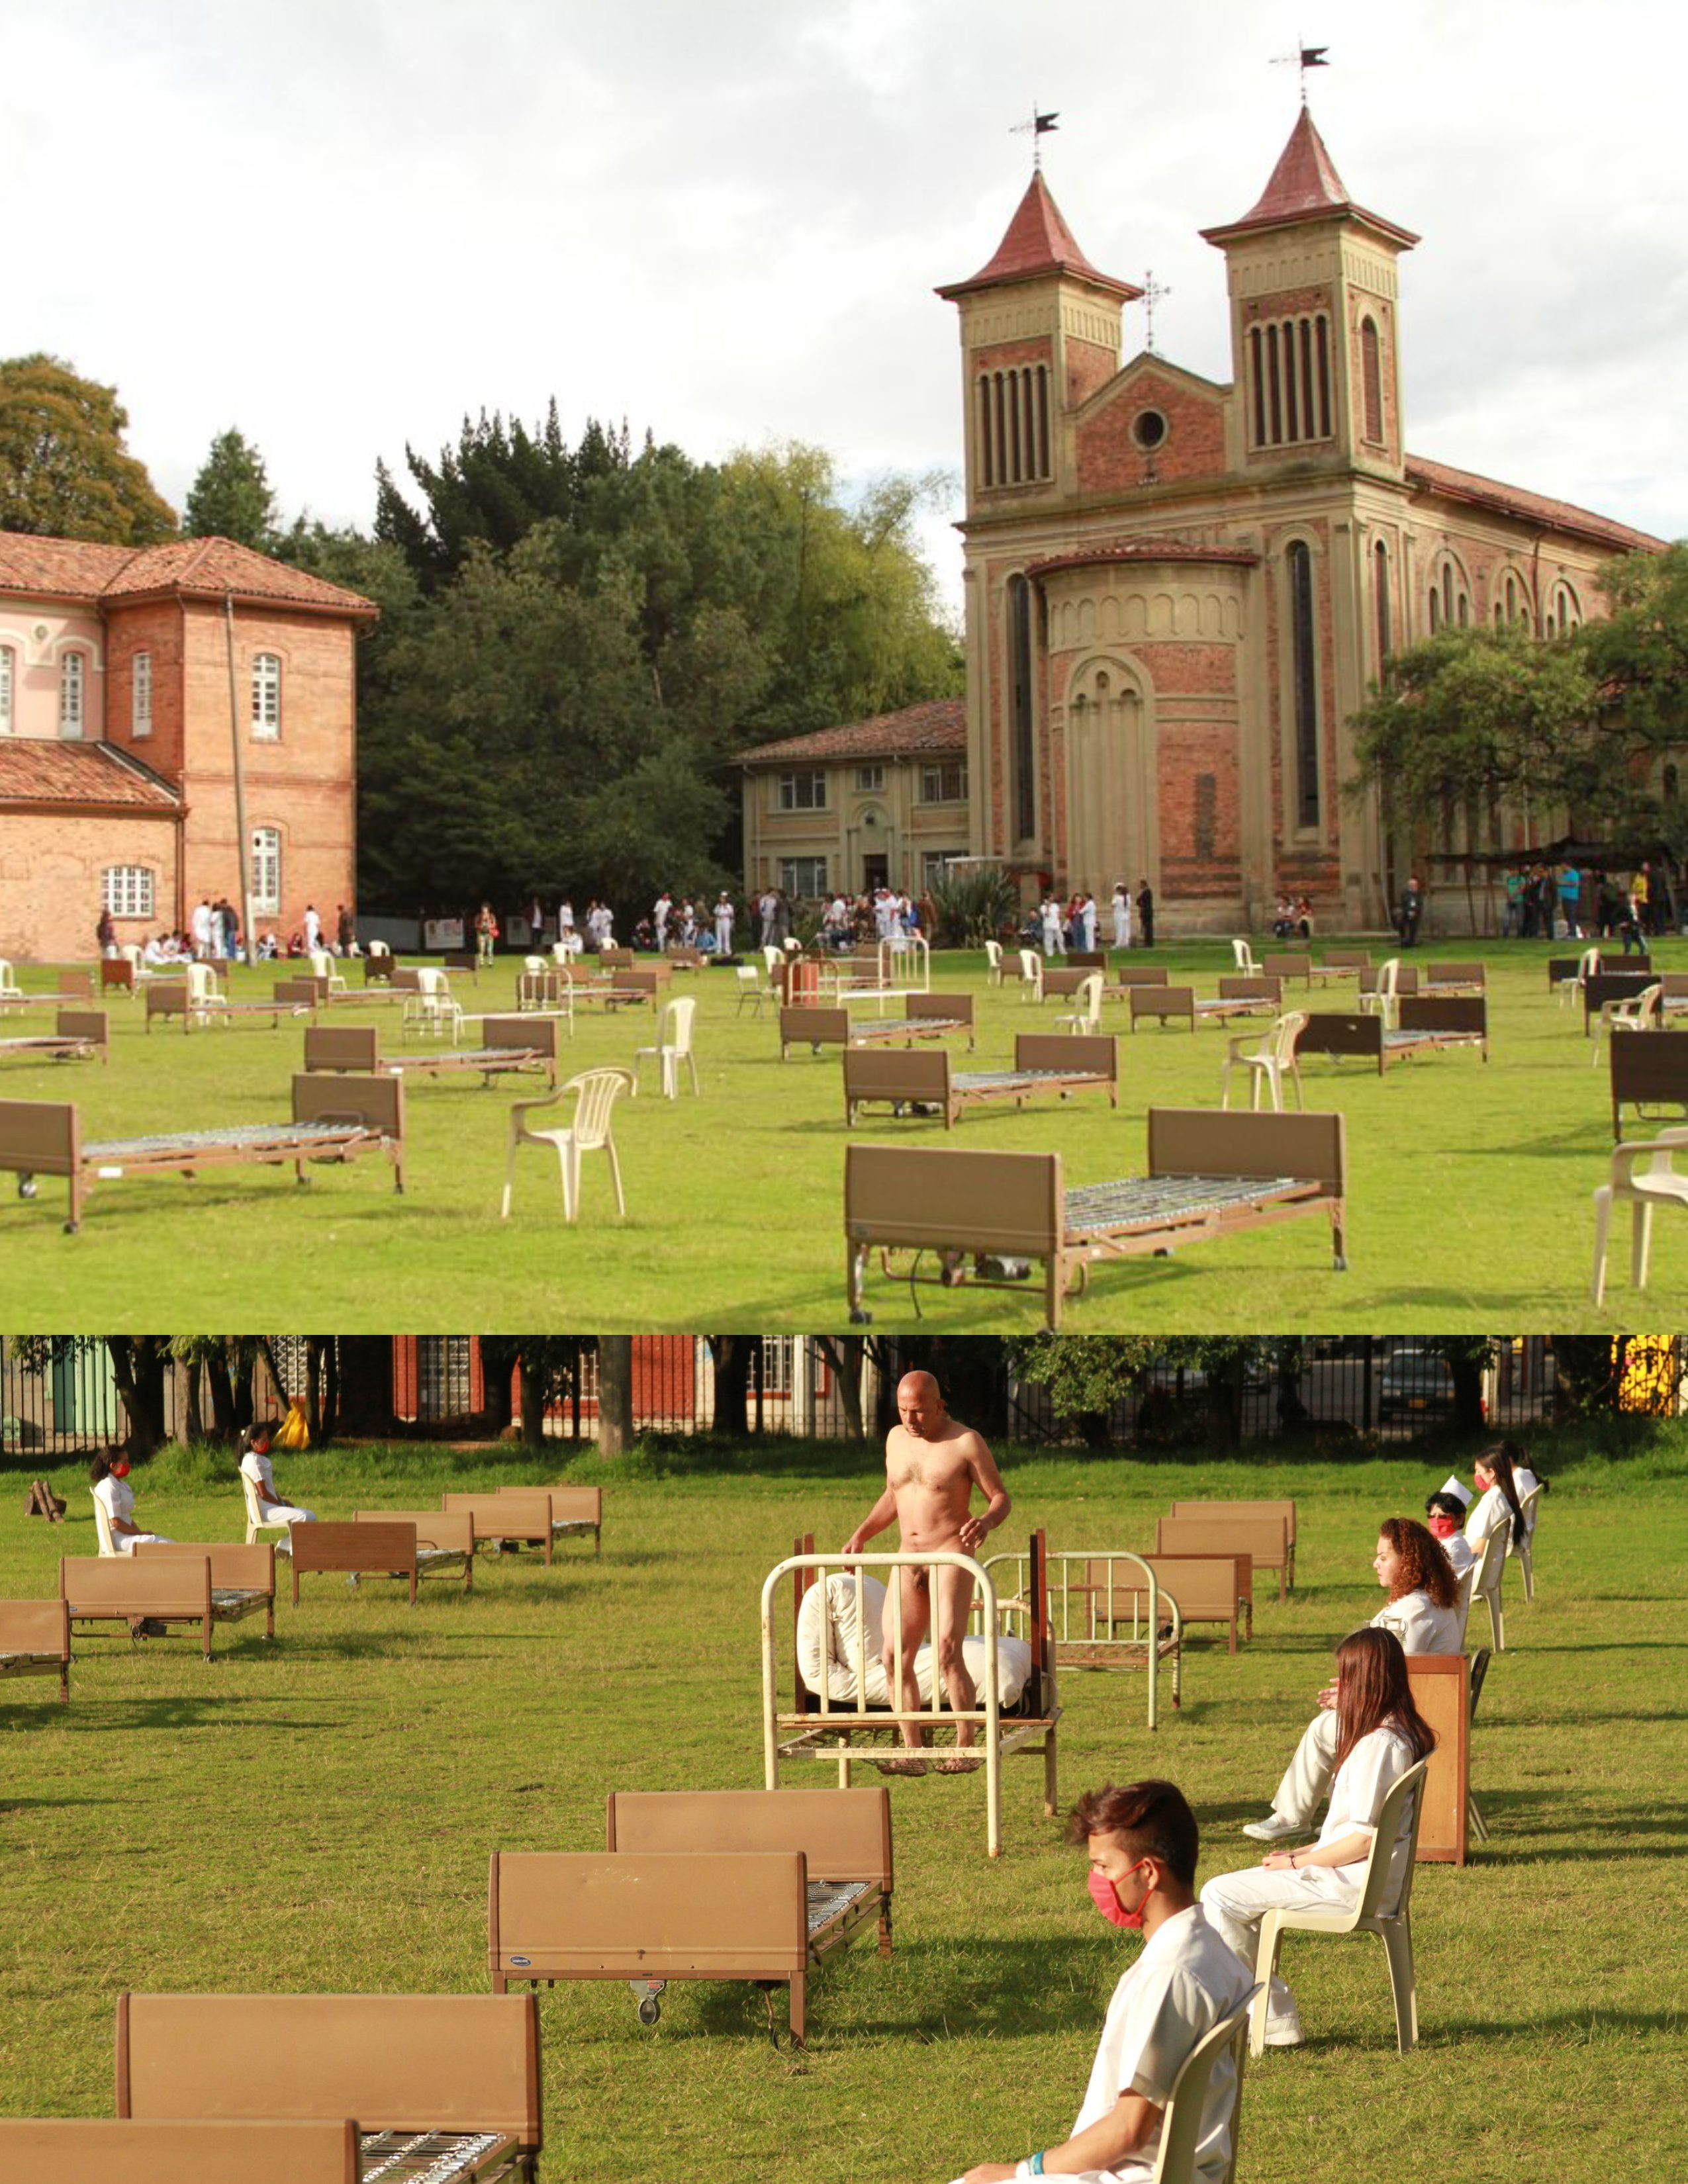
\includegraphics[height=\paperheight]{hortua-inhospitalaria.jpg}
        };
        \node[anchor=south,text width=0.85\paperwidth,align=center,fill=white,fill opacity=0.9,text opacity=1,inner sep=15pt] at ([yshift=3cm]current page.south) {
            \small \textbf{Figura 1.1:} Hortúa Inhospitalaria, 2017. Performance de David Lozano.\\[0.3em]
            \href{https://david-lozano.org/work/hortua-inhospitalaria}{Copyright David Lozano}
        };
    \end{tikzpicture}
    \caption{Hortúa Inhospitalaria, 2017. Performance de David Lozano.}
    \label{fig:david_lozano_hortua}
\end{figure}

\textcolor{edit30sept}{Samain afirma que “las imágenes, esa colección, ese conjunto de archivos digitales con intención, que tienen una intención, eso genera como una potencia que permite, aún estando en otro momento, en otro tiempo, en otro contexto, volver a ellas y mirarlas” (Samain, 2016, p. 105), en el archivo de Margarita funciona precisamente como este tipo de “conjunto con intención”. Las operaciones de montaje —poner “una imagen con otra”— revelan narrativas no explícitas, pero profundamente significativas, sobre las condiciones de habitabilidad, resistencia y supervivencia en el hospital.}

La crisis del Hospital San Juan de Dios (HSJD) emerge como un laboratorio social donde el diseño y la creación interactiva permiten explorar las dinámicas de transformación institucional, memoria colectiva y resistencia ciudadana. Este estudio trasciende la mera indagación documental o artística para analizar cómo diversas acciones simbólicas, argumentales y estéticas evidencian una intensa producción visual en torno a dicha crisis. Los registros de estas acciones configuran un corpus de imágenes que posibilita interpretar tanto los síntomas visuales de la crisis sistémica como el deterioro arquitectónico y patrimonial en su interacción con el drama humano y social.

El caso del HSJD resulta emblemático en el contexto de las crisis institucionales derivadas de las transformaciones masivas en los sistemas de salud pública. Surge entonces la pregunta: ¿cómo comprender, explicar e interpretar los registros visuales y las obras que actúan como evidencias del drama humano y de la defensa de un bien público?

\textcolor{edit30sept}{Estas evidencias, que denominamos imagen-síntoma, constituyen presencias disruptivas que irrumpen en el curso \textcolor{edit30sept}{normativizado} de la representación visual. Se trata de supervivencias, latencias y reapariciones que habitan las imágenes y desafían el régimen escópico dominante: una mirada que se torna paisaje contemplativo y desvincula la acción crítica. La metodología aplicada a esta colección visual de memoria social permite abordar el fenómeno a través de la imagen, generando un espacio para interpelar y activar la percepción más allá de lo meramente representacional.}

El concepto de imagen-síntoma\footnote{\begin{quote}La idea de la imagen como síntoma, tomada por Didi-Huberman de Freud y aplicada al campo de la historia del arte, reconoce las diferencias entre disciplinas y experiencias. Sin embargo, el uso del carácter sintomático de la imagen en la historia del arte mantiene paralelismos con el análisis de los sueños, aunque aquí se utiliza para nombrar la perturbación que lo visual causa dentro de lo visible \parencite[p. 37]{VegaArevalo2017}\end{quote}} resulta fundamental para comprender cómo las representaciones visuales del HSJD trascienden la mera documentación para convertirse en manifestaciones de tensiones sociales más profundas. Como señala Didi-Huberman:

\begin{quote}
Si la imagen es un síntoma —en el sentido crítico y no clínico del término—, si la imagen es un malestar en la representación, es porque indica un futuro de la representación, un futuro que no sabemos aún leer ni, incluso, describir \parencite[p. 177]{DidiHuberman2011}.
\end{quote}

Este estudio profundiza en el papel de la imagen como medio privilegiado para la contemplación de los fenómenos sociales, ofreciendo nuevas perspectivas que contribuyen al debate sobre el rol del arte y el diseño en los procesos de cambio social y en la construcción de memoria colectiva.

El diseño, entendido como práctica crítica y performática, permite develar las capas de significado ocultas en los registros visuales. No se trata únicamente de documentar, sino de construir narrativas que revelen las tensiones sociales subyacentes. Las imágenes del HSJD se transforman así en interfaces de memoria, donde cada fragmento, ruina y registro artístico opera como un nodo de información compleja.

\textcolor{edit30sept}{En este marco, se propone el concepto de \textit{meta-composición estética y documental} para nombrar el tránsito del análisis de la imagen al dispositivo que la contiene y la reescribe críticamente. Se concibe como una operación de segundo orden que, mediante el \textit{montaje}, articula archivos, escenas, anacronismos e \textit{imagen-síntoma} en una composición que reflexiona sobre su propio proceso de documentación y producción de sentido. Esta operación no busca clausurar significados, sino activar la experiencia crítica del lector/espectador, integrando procedimientos de archivo, selección y montaje en un continuum estético-documental coherente con los objetivos de esta investigación.}

\textcolor{edit30sept}{Desde esta perspectiva, el diseño se concibe como una herramienta estratégica para articular un dispositivo de activación memorial: un mecanismo que, a través de obras artísticas y registros visuales, cataliza procesos orientados a:}

\begin{itemize}
\item Desarticular las narrativas oficiales sobre el abandono institucional;
\item Visibilizar las experiencias de trabajadores y comunidades afectadas;
\item Generar nuevas formas de comprensión y elaboración del conflicto social.
\end{itemize}

\textcolor{edit30sept}{En el ensayo \textit{El derecho a mirar}, Nicholas Mirzoeff define la visualidad no como una mera percepción óptica, sino como un conjunto de relaciones que combinan la información, la imaginación y la reflexión para generar un panorama tanto físico como psíquico. Esta concepción desborda el sentido técnico de “ver” y la aproxima a una práctica discursiva que produce realidad al articular formas de conocimiento, afecto y poder. Desde esta perspectiva, dichas tres dimensiones pueden entenderse como \textit{métodos de visualización}, en tanto configuran operaciones epistemológicas mediante las cuales se construyen modos de percepción, interpretación y representación del mundo.}

\begin{quote}
\textcolor{edit30sept}{A pesar de su nombre, la visualidad no está únicamente compuesta por percepciones visuales en un sentido físico, sino que engloba un conjunto de relaciones en las que se combinan la información, la imaginación y la reflexión para generar un panorama tanto físico como psíquico \parencite{Mirzoeff2016}.}
\end{quote}


\textcolor{edit30sept}{La información, la imaginación y la reflexión operan aquí como tres métodos de visualización interdependientes que orientan el desarrollo analítico de esta investigación. Nombrarlas métodos implica reconocer su carácter procesual y activo: no describen únicamente lo que la visualidad contiene, sino cómo se produce. La información organiza y materializa los datos visibles; la imaginación interviene como potencia de creación y recomposición de lo real; y la reflexión introduce la distancia crítica que permite reconfigurar la mirada y cuestionar los regímenes de visibilidad establecidos. Así, estos tres métodos de visualización atraviesan el análisis propuesto en esta investigación, orientando la lectura de las imágenes no como objetos estáticos, sino como campos de experiencia donde se interrelacionan el conocimiento, la sensibilidad y la crítica.}

\textcolor{edit30sept}{Más que categorías cerradas (la información, la imaginación y la reflexión), constituyen dinámicas de pensamiento y percepción que atraviesan los distintos niveles de lectura del archivo visual del HSJD. En este sentido, la imagen-síntoma se concibe como un espacio donde estos procesos convergen, permitiendo que la representación trascienda su dimensión documental para devenir en una herramienta de interpelación al régimen escópico dominante.}


\section*{Contextualización histórica}

El Hospital San Juan de Dios (HSJD) de Bogotá, fundado en 1723, se estableció como un centro pionero de atención médica y asistencia social para la población vulnerable. Durante casi tres siglos, esta institución se consolidó como un referente fundamental de la salud pública en Colombia, destacándose tanto por su labor asistencial como por su rol en la formación de profesionales de la salud. Sin embargo, la década de 1990 marcó el inicio de una serie de crisis institucionales y financieras que culminarían en su cierre.

El año 2001 representa un punto de inflexión en la historia del hospital, cuando "3.640 personas quedaron desempleadas, y aproximadamente 1.500 trabajadores no recibieron la liquidación correspondiente por sus años de servicio" \parencite{Castiblanco2017}. Este acontecimiento catalizó múltiples formas de resistencia ciudadana que trascendieron la mera reivindicación laboral, evidenciando un complejo entramado de problemáticas sociales.

La crisis del HSJD tiene raíces profundas que anteceden al cese de sus operaciones. Según el investigador Mario Hernández, especialista en historia de la medicina, las décadas de 1970 y 1980 marcaron el inicio de la crisis de los Estados de Bienestar, período caracterizado por la implementación de políticas neoliberales. La presión por incorporar los servicios de salud a las dinámicas de mercado impulsó una transformación institucional que el hospital, originalmente concebido bajo un modelo de beneficencia, no logró asimilar exitosamente. Esta transición fallida se manifestó en el deterioro progresivo de su infraestructura patrimonial, aunque el hospital mantuvo su función asistencial hasta su último día de operación.

Paralelamente a las iniciativas institucionales para su reapertura, emergieron diversas expresiones de resistencia social, manifestaciones artísticas y acciones conmemorativas que abordaron la complejidad del fenómeno. \textcolor{edit30sept}{Es así como} esta investigación se centra en el análisis de la construcción de sentido a través de obras e imágenes artísticas, estéticas y poéticas no funcionales.

\subsubsection*{Exhibición y creación}

El HSJD se ha convertido en un punto focal para diversos campos disciplinares, atrayendo la atención de urbanistas, antropólogos y artistas plásticos, quienes encuentran en sus espacios un rico territorio para la reflexión y la creación. Este caso paradigmático ha catalizado el debate público sobre la salud como derecho fundamental, manifestándose a través de diversas prácticas disciplinares y expresiones simbólicas.

A partir de 2007, se observa una proliferación sistemática de manifestaciones artísticas que abordan explícitamente la problemática del HSJD. Desde entonces, se han producido y exhibido con regularidad casi anual obras artísticas, intervenciones estéticas y ocupaciones arquitectónicas relacionadas con esta situación.

\begin{table}[htbp]
\centering
\begin{tabular}{|l|l|l|}
\hline
\textbf{Año} & \textbf{Artista} & \textbf{Obra} \\ \hline
2007 & María Elvira Escallón & En estado de coma \\ \hline
2011 & Nicolas Van Hemelryck & San Juan sin Dios \\ \hline
2013 & Juan Camilo Ahumada & Tiempo de dios (guión para teatro) \\ \hline
2015 & Fredy Alzate & Quiste \\ \hline
2015 & Alexandra Mccormick & Potenciales Evocados para aplicaciones clínicas \\ \hline
2015 & Víctor Garcés & Juan N de Dios \\ \hline
2015 & Jenniffer Duarte & Didácticos para una sala de espera \\ \hline
2015 & Ana Karina Moreno & Una más de las resistencias \\ \hline
2015 & Nathaly Rubio & Lo mejor es que nos olvidamos \\ \hline
2015 & Harold Ortiz & Sala de espera \\ \hline
2015 & Alejandro Arango & Egotherapy \\ \hline
2015 & David Lozano & Hortua inhospitalario \\ \hline
2017 & Luisa Fernanda Vela & Al margen \\ \hline
\end{tabular}
\caption{Obras y artistas relacionados con el HSJD, 2007-2017.}
\label{tabla:obras_artistas}
\end{table}

Complementando estas obras, se han realizado diversas activaciones in situ, incluyendo la \textit{Cumbre Mundial de Arte y Cultura para la Paz} y \textit{Time Bag Bogotá} \parencite{IDARTES2015}. Esta tendencia ha continuado más allá del marco temporal de este estudio, con eventos como la \textit{Feria del Millón} (2021), \textit{Siga esta es su casa} (2022) y \textit{La pulsión de la vida} - Activaciones sociales del IDPC.

\section*{Planteamiento del problema}

La crisis del Hospital San Juan de Dios (HSJD) de Bogotá plantea interrogantes fundamentales sobre la respuesta social ante el abandono institucional: ¿Qué acciones tomar? ¿Permanecer, partir, resistir? ¿Por qué y hasta cuándo? Si bien el egreso del último paciente en 2001 marcó un hito significativo, este evento no representó el cierre definitivo del hospital. El proceso de deterioro institucional había iniciado años antes, y las gestiones para su liquidación y eventual reapertura se han extendido por décadas, situando al HSJD en un peculiar estado de latencia activa.

Paralelamente a los esfuerzos institucionales, el HSJD ha sido escenario de diversas manifestaciones de resistencia social, investigación académica y expresión artística que abordan la complejidad del fenómeno. Mientras el hospital experimentaba su desmaterialización funcional, emergían simultáneamente acciones de construcción de sentido en sus dimensiones patrimoniales, estéticas y poéticas. Este contexto suscita interrogantes cruciales sobre la naturaleza de la imagen artística y su capacidad para expresar la crisis y resistencia en el HSJD.

Para analizar los registros gráficos y audiovisuales —que incluyen procesos de creación artística, instalaciones \textit{in situ}, performances y una obra de dramaturgia— se adopta el concepto de \textit{imagen-síntoma}. Este enfoque trasciende el análisis formal de las imágenes para examinar su capacidad de revelar manifestaciones del drama humano y social, considerando que estos registros contienen signos icónicos e indicios de la imaginación social colectiva.

El \textit{corpus} de imágenes relacionadas con el HSJD exhibe recurrencias discursivas provenientes de diversos ámbitos de participación, evidenciando tanto la crisis como las respuestas críticas ante situaciones que generan más interrogantes que certezas. Estas representaciones visuales constituyen un discurso que demanda una interpretación desde una perspectiva crítica y multidimensional.

En este contexto, surge la pregunta central: ¿De qué manera las representaciones visuales y artísticas de la crisis del HSJD contribuyen a la construcción de la memoria colectiva y al entendimiento de problemáticas sociales sistémicas? ¿Cómo pueden estas representaciones ser reinterpretadas, mediante el montaje y la experiencia visual, para generar narrativas transformadoras que estimulen el debate social?. \textcolor{edit30sept}{Metodológicamente, la \textit{meta-composición estética y documental} opera como respuesta al problema de investigación: permite reconfigurar el \textit{corpus} visual en escenas montadas que hacen visible el \textit{síntoma} y el \textit{anacronismo} como tensiones productivas, habilitando una construcción de sentido que excede la mera acumulación de evidencias y propone una forma reflexiva de organización de la memoria visual.}

De esta interrogante principal se desprenden tres preguntas orientadoras:

\begin{enumerate}
    \item \textbf{¿Cómo se representa la crisis y la resistencia en el HSJD a través del arte y la memoria visual?}

    \item \textbf{¿Qué significado adquiere la imagen artística en el contexto de crisis social y resistencia?}

    \item \textbf{¿Cómo las obras visuales sobre el HSJD establecen una relación simbólica entre el entorno social y el espectador?}
\end{enumerate}

\section*{Justificación y relevancia}

La crisis del Hospital San Juan de Dios (HSJD) constituye una problemática sistémica donde convergen múltiples dimensiones interconectadas: económicas, administrativas, sociales, políticas y culturales. Desde la perspectiva del diseño y la creación interactiva, resulta pertinente abordar estas problemáticas sociales complejas mediante enfoques y metodologías innovadoras, especialmente en el actual contexto colombiano de construcción de paz. En este escenario, la transformación social requiere trascender la mera resolución del conflicto para atender otros ámbitos del bienestar social \parencite[p. 313]{Capra1998}.

El presente estudio se fundamenta en un corpus documental que comprende más de 800 registros visuales\footnote{Ver Apéndice B para más detalles.}, cuidadosamente seleccionados de producciones académicas y artísticas que abordan la crisis y cierre del HSJD. Resulta significativo observar la correlación temporal entre los momentos más álgidos de la crisis hospitalaria y el incremento en la producción artística, fenómeno que coincide además con una intensificación en la cobertura mediática del caso por parte de los principales medios de comunicación bogotanos.

Este fenómeno visual-documental demuestra cómo la crisis del HSJD ha trascendido su dimensión institucional para convertirse en un símbolo de resistencia y reflexión sobre el estado de la salud pública en Colombia. La abundancia y diversidad de registros visuales evidencia la necesidad de analizar cómo estas representaciones contribuyen tanto a la construcción de memoria colectiva como a la comprensión de fenómenos sociales complejos desde la perspectiva del pensamiento visual y la creación interactiva.

La implementación de la Ley 100 tuvo como una de sus principales consecuencias la agudización de la crisis en los hospitales públicos, al permitir una retirada progresiva del Estado frente a sus responsabilidades con la salud de los colombianos y dejar a la deriva las entidades de carácter oficial \parencite{Castiblanco2017}. Diversos estudios han documentado cómo, tras la publicación de esta ley en 1993, el hospital entró en una rápida fase de decadencia.

Esta situación provocó la pérdida de hogares y bienes materiales de numerosos empleados y sus familias, lo que derivó en la "toma" del Hospital. Paralelamente, este hecho marcó el inicio de una extensa batalla jurídica que, incluso en 2015, más de catorce años después, continuaba vigente \parencite{Orlando2015}. La lucha por los derechos laborales negados durante la precipitada e insatisfactoria liquidación de la Fundación San Juan de Dios se ha extendido ya por dos décadas.

Es importante señalar que, según la documentación institucional, el hospital nunca ha dejado de existir formalmente. De hecho, al momento de redactar este informe, se encuentra en desarrollo un proyecto de «intervención integral de 7 de los 17 edificios de mayor valor patrimonial del Complejo Hospitalario, así como de los espacios emblemáticos del costado nororiental, con el fin de consolidar la primera etapa de la reactivación funcional de este hospital».